\subsection{Impact of Congestion Control} \label{s:robust:cross}\label{s:eval:cc}
How does our choice of congestion control impact our results? 
We first verify that \name indeed runs congestion control algorithms appropriately.
\begin{figure}
    \centering
    \begin{subfigure}[b]{0.5\textwidth}
\begin{knitrout}
\definecolor{shadecolor}{rgb}{0.969, 0.969, 0.969}\color{fgcolor}
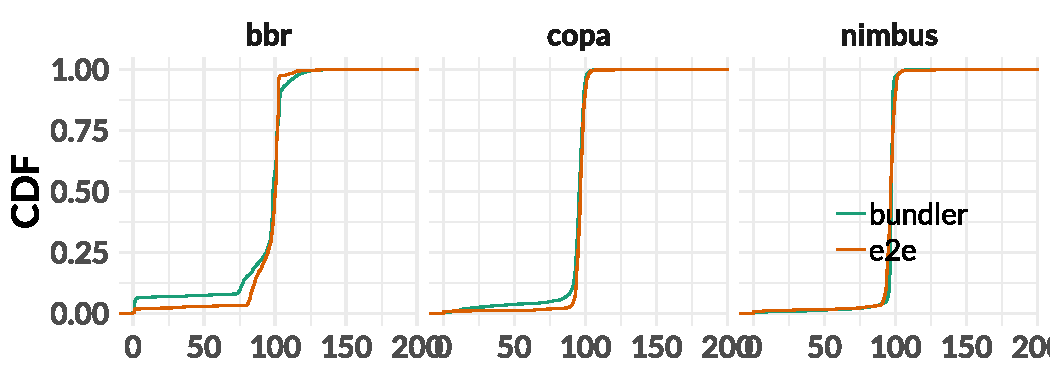
\includegraphics[width=\maxwidth]{figure/eval:tput-delay:a-1} 

\end{knitrout}
    \caption{Throughput (in Mbit/s) Comparison.}\label{fig:eval:tputdelay:a}
    \end{subfigure}
    \begin{subfigure}[b]{0.5\textwidth}
\begin{knitrout}
\definecolor{shadecolor}{rgb}{0.969, 0.969, 0.969}\color{fgcolor}
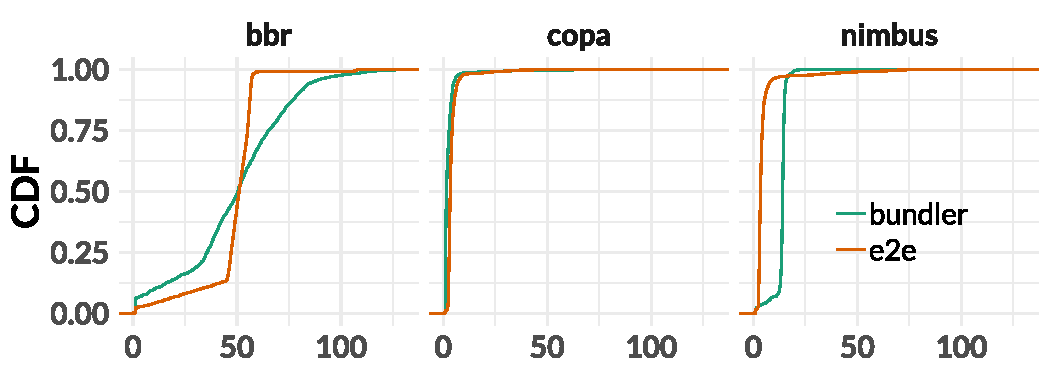
\includegraphics[width=\maxwidth]{figure/eval:tput-delay:b-1} 

\end{knitrout}
    \caption{Delay (in ms) Comparison.}\label{fig:eval:tputdelay:b}
    \end{subfigure}

    \caption{\name can shape underlying Cubic flows so they assume the characteristics of \name's congestion control algorithm.}
    \label{fig:eval:tputdelay}
\end{figure}

Figure~\ref{fig:eval:tputdelay} shows that for two of the three congestion control algorithms we evaluate --- Copa~\cite{copa} and Nimbus~\cite{nimbus} --- the throughput (in Figure~\ref{fig:eval:tputdelay:a}) and queueing delay (in Figure~\ref{fig:eval:tputdelay:b}) distributions over a one-minute experiment are similar to the same algorithm running at the end-host (\ie without \name).

BBR's~\cite{bbr} delay distribution suffers because of its interaction with the end-to-end congestion control. When BBR enters its \texttt{PROBE\_RTT} mode by setting a congestion window of $4$ packets, end-host implementations simply stop transmitting.
However, with \name the end-host implementation is Cubic; it continues probing for bandwidth until the \inbox is forced to drop packets.

\name is compatible with multiple endhost congestion control algorithms\footnote{We omit a figure for brevity.}.
When we configure endhosts to use BBR\footnote{We use the BBR implementation provided in Linux $4.13$.} (instead of Cubic as above), \name's benefits remain: \name achieves 58\% lower FCTs in the median.
This is primarily because in the \baseline using BBR causes endhosts to achieve 66\% worse median slowdown ($1.62$ with Cubic to $2.68$ with BBR); \name's slowdown is only 5\% worse when endhosts use BBR ($1.08$ with Cubic to $1.14$ with BBR).

\paragrapha{Self-Inflicted Delays} Correct congestion control behavior is crucial to achieving low FCTs.
In Figure~\ref{fig:eval:cc} we compare three congestion control protocols to the Baseline: BBR~\cite{bbr}, Nimbus~\cite{nimbus}, and Copa~\cite{copa}.
In this scenario, it is important to control delays in the bottleneck queue, since it is FIFO scheduled and therefore queued packets from short requests must wait behind those from longer requests. Nimbus and BBR both maintain slightly higher queueing delays at the bottleneck link, and thus they achieve higher median FCTs \an{numbers}. 
Nimbus, which is slightly more aggressive than Copa, induces a higher queue build up at the bottleneck, and a smaller queue build up at the \name, when compared to Copa. It therefore results in a higher median FCT than Copa, though still providing significant benefits over the baseline. 
BBR, however is even more aggressive and cannot maintain sufficient queuing at the \name to provide enough benefits.

\radhika{Also, no way to further improve BBR?}
\an{try to understand bbr results}

%\radhika{might be interesting to have another line that shows what happens when \name uses Cubic, and how it can break things.}
%\an{I don't think we can run a meaningful cubic experiment since the implementation looks carefully at measurements (loss, out-of-order deliveries) that we don't precisely measure}
%\an{try running a cubic experiment}

\begin{figure}
    \centering
\begin{knitrout}
\definecolor{shadecolor}{rgb}{0.969, 0.969, 0.969}\color{fgcolor}
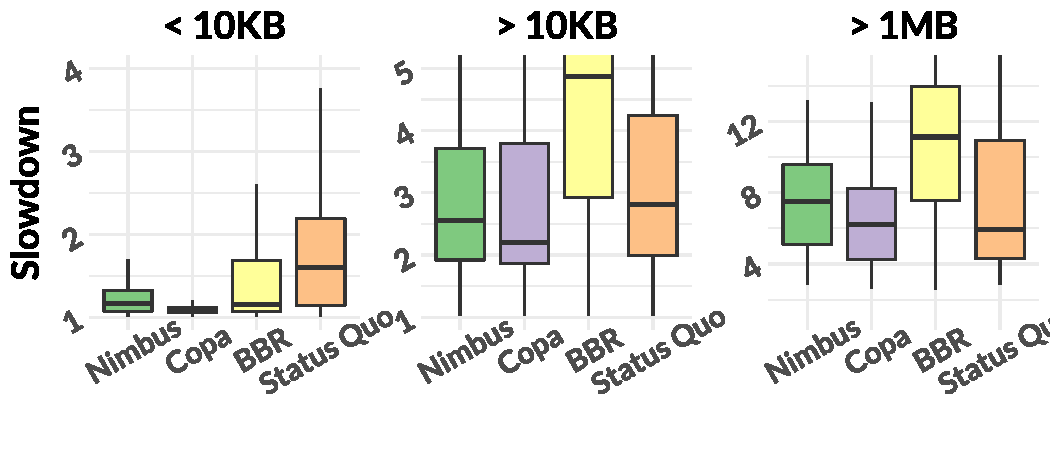
\includegraphics[width=\maxwidth]{figure/eval:cc-1} 

\end{knitrout}
    \caption{Choosing a congestion control algorithm at \name remains important, just as it is at the end-host. Note the different y-axis scales for each group of request sizes.}
    \label{fig:eval:cc}
\end{figure}
\newcommand{\ccCopaMedian}{}
\newcommand{\ccNimbusMedian}{}
\newcommand{\ccBBRMedian}{}
\newcommand{\ccBaselineMedian}{}


Meanwhile, the characteristics of other traffic --- not part of the traffic aggregate \name controls --- on the link can force \name's congestion controller to behave more aggressively in order to remain competitive in the bottleneck link. This would reduce the amount of queue build up at the \name, thus reducing its benefits.

\begin{figure}
    \centering
\begin{knitrout}
\definecolor{shadecolor}{rgb}{0.969, 0.969, 0.969}\color{fgcolor}
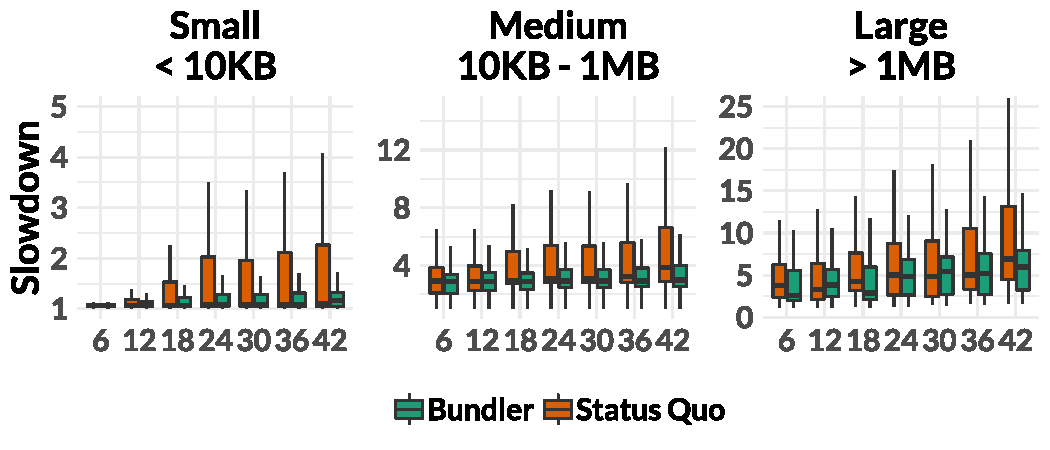
\includegraphics[width=\maxwidth]{figure/robust_cr-inelastic-1} 

\end{knitrout}
    \caption{Against cross traffic comprising of short lived flows. \name offers 48Mbps of load to the bottleneck queue. The cross traffic's offered load increases along the x-axis, while \name{}'s offered load remains fixed.}
    \label{fig:robust:cr-inelastic}
\end{figure}

\paragrapha{Inelastic Cross Traffic} We first consider the case of \emph{inelastic} cross traffic; that is, traffic that does not respond to queue-size fluctuations.
For example, traffic primarily comprised of short web requests has the inelastic property because regardless of what \name's congestion controller (or any end-to-end congestion controller) does, the component short requests, which remain in TCP slow start for their entirety, will occupy some fraction of the bottleneck link capacity.
In this case, the congestion controller must yield bandwidth to the cross traffic, but can still maintain low delays at the bottleneck link.

We can see this phenomenon in action in Figure~\ref{fig:robust:cr-inelastic}. 
Each of the congestion control algorithms we evaluate sacrifice (to varying degrees) bandwidth in reaction to the cross traffic, which hurts the FCTs of the larger requests.
However, the scheduling policy apportions the remaining bandwidth to the short flows, so there is still an improvement in FCTs at the median.

\begin{figure}
    \centering
    \begin{subfigure}[b]{0.5\textwidth}
\begin{knitrout}
\definecolor{shadecolor}{rgb}{0.969, 0.969, 0.969}\color{fgcolor}
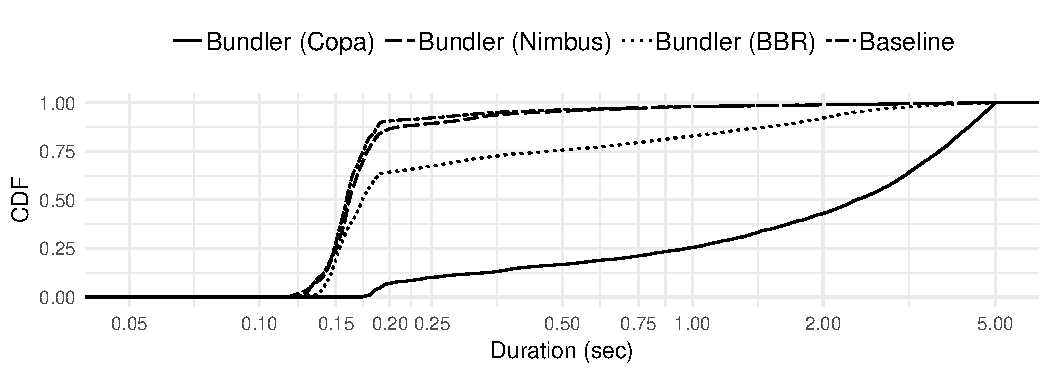
\includegraphics[width=\maxwidth]{figure/robust:cr-elastic:a-1} 

\end{knitrout}
    \caption{Congestion controllers from \S\ref{s:eval}.}\label{fig:robust:cr-elastic:a}
    \end{subfigure}
    \begin{subfigure}[b]{0.5\textwidth}
\begin{knitrout}
\definecolor{shadecolor}{rgb}{0.969, 0.969, 0.969}\color{fgcolor}
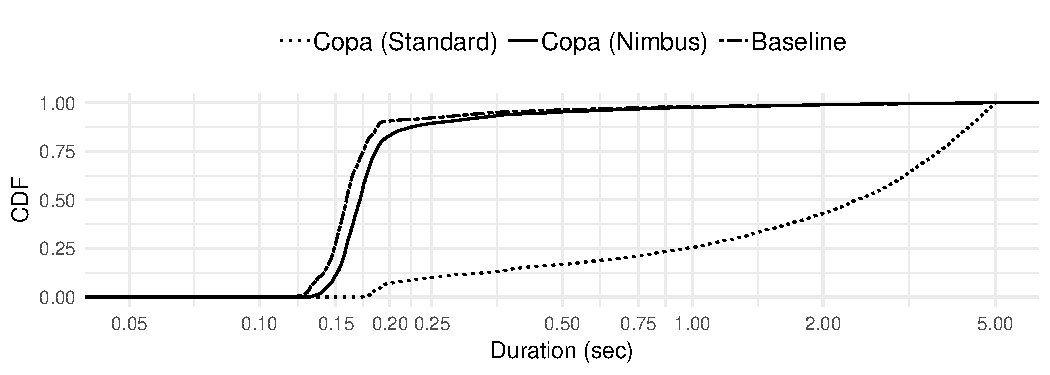
\includegraphics[width=\maxwidth]{figure/robust:cr-elastic:b-1} 

\end{knitrout}
    \caption{Alternate configuration -- Copa uses Nimbus's elasticity detector.}\label{fig:robust:cr-elastic:b}
    \end{subfigure}

    \caption{Elastic cross traffic.}
    \label{fig:robust:cr-elastic}
\end{figure}

\paragrapha{Elastic Cross Traffic} Elastic cross traffic, which fills the bottleneck link's buffer, is the worst-case scenario for \name.
The congestion controller must push packets into the bottleneck queue to compete fairly, and thus it cannot retain packets at the \inbox to schedule.
As a result, we expect performance to be no better than the baseline.
We indeed see this in Figure~\ref{fig:robust:cr-elastic}.

\an{In this experiment, Copa, primarily a delay-based algorithm, cannot adequately detect the presence of competing elastic traffic and ``mode-switch'' to its competitive mode. 
%When we modify Copa to use Nimbus's elasticity detector (Figure~\ref{fig:robust:cr-elastic}), its performance matches the baseline.
}

\begin{figure}
    \centering
\begin{knitrout}
\definecolor{shadecolor}{rgb}{0.969, 0.969, 0.969}\color{fgcolor}
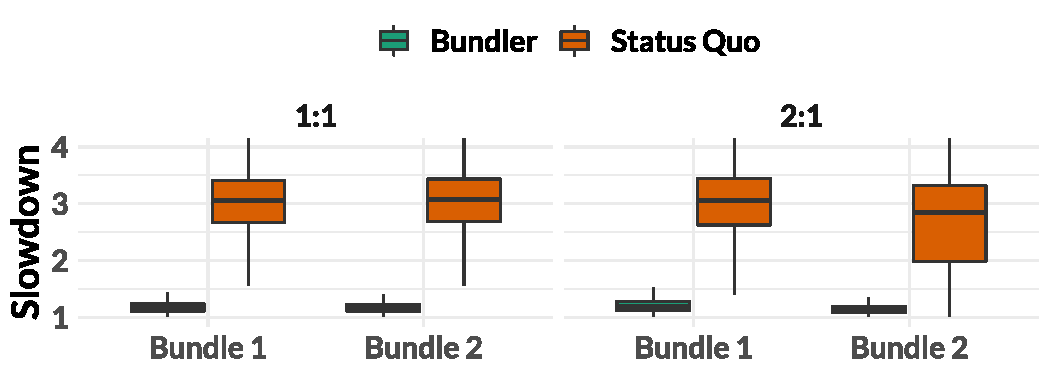
\includegraphics[width=\maxwidth]{figure/robust_twobundler-1} 

\end{knitrout}
    \caption{Competing traffic bundles. In both cases, the aggregate offered load is 84Mbps, as in Figure~\ref{fig:eval:best}. For "1:1", we evenly split the offered load between the two Bundles; for "2:1", one bundle has twice the offered load of the other. In both cases, each bundle observes improved median FCT compared to its performance in the baseline scenario.}
    \label{fig:robust:twobundler}
\end{figure}

\paragrapha{Competing Bundles} \name's improvements return once competing traffic starts using \name as well. In Figure~\ref{fig:robust:twobundler}, we show the performance of each of two bundles of traffic competing in the same bottleneck link. 
Despite both bundles containing persistently backlogged flows, just as in Figure~\ref{fig:robust:cr-elastic}, here \name improves the FCTs of both bundles independently.

\cut{
\subsection{Path Characteristics}\label{s:robust:path}
\an{should these go in ``microbenchmarks'' in \S\ref{s:measurement}?} \radhika{i don't think so}
\begin{outline}
\1 Different RTTs
\1 Different bandwidths
\end{outline}
}
